\begin{frame}{}
    \LARGE Generative AI for Science: \textbf{Generative Models in Physical Simulations}
\end{frame}

\begin{frame}[allowframebreaks]{Generative Models in Physical Simulations}
    \begin{figure}
        \centering
        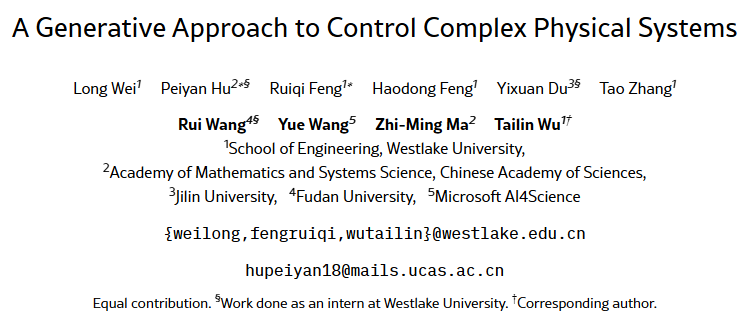
\includegraphics[height=0.9\textheight,width=1\textwidth,keepaspectratio]{images/science/generative-models-cover.png}
    \end{figure}

    \framebreak

    \textbf{Why use Generative Models for Physical Simulations?}

    \begin{itemize}
        \item Simulating things like fluids or materials is slow and needs a lot of computer power.
        \item Traditional methods solve tough math equations (PDEs) step by step, which takes time.
        \item Generative models can learn how these systems behave, so we can get results much faster.
        \item This means scientists can try out more ideas and make discoveries quicker.
    \end{itemize}

    \framebreak

    \textbf{What can Generative AI do in Simulations?}
    \begin{itemize}
        \item \textbf{Faster Simulations:} Quickly create realistic simulations without heavy calculations.
        \item \textbf{Learn from Data:} Use real data to make new, believable scenarios.
        \item \textbf{Work at Different Scales:} Model things from tiny atoms to big objects.
        \item \textbf{Predict the Future:} Guess what might happen next in a system.
        \item \textbf{Mix with Experiments:} Combine with real-world data to make better predictions.
        \item \textbf{Help Scientists and Engineers:} Make it easier to test new ideas and designs.
    \end{itemize}

    \framebreak
    \begin{figure}
        \centering
        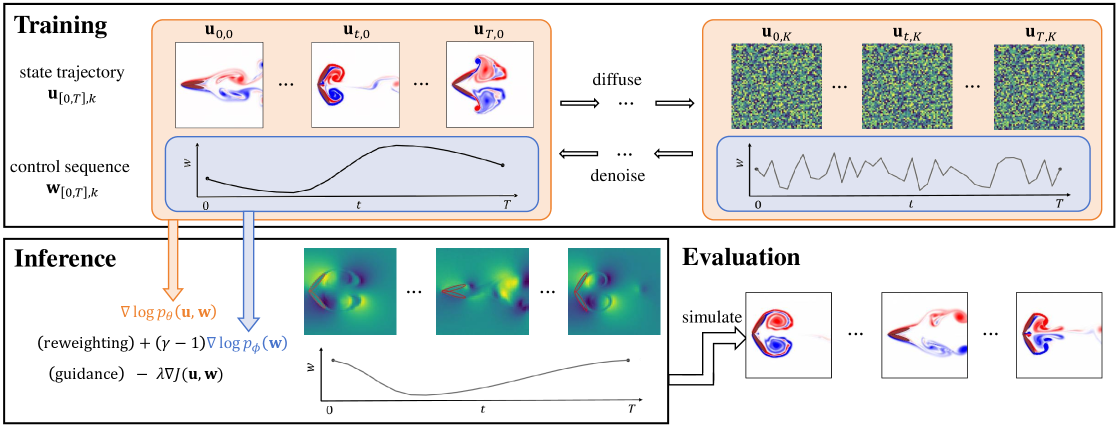
\includegraphics[height=0.85\textheight,width=1\textwidth,keepaspectratio]{images/science/generative-models-diffphycon.png}
        \caption*{DiffPhyCon: A tool that uses generative models to simulate physical systems.}
    \end{figure}

    \framebreak
    \begin{figure}
        \centering
        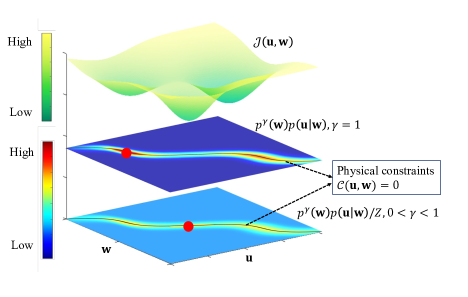
\includegraphics[height=0.65\textheight,width=1\textwidth,keepaspectratio]{images/science/generative-models-intuit.png}
        \caption*{How prior reweighting helps: By adjusting how we sample, we can find better solutions in our simulations.}
    \end{figure}

    \framebreak
    \begin{figure}
        \centering
        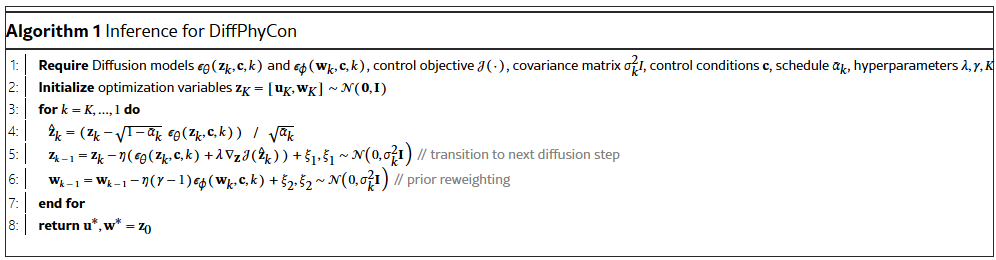
\includegraphics[height=0.9\textheight,width=1.05\textwidth,keepaspectratio]{images/science/generative-models-algo.png}
    \end{figure}

    \framebreak
    \begin{figure}
        \centering
        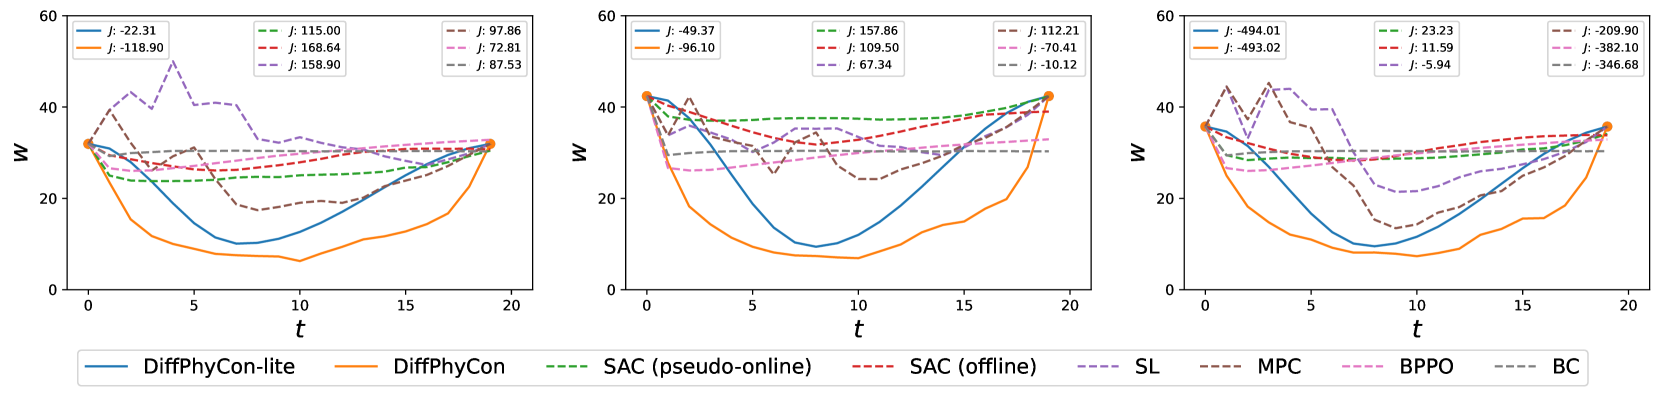
\includegraphics[height=0.8\textheight,width=1.05\textwidth,keepaspectratio]{images/science/generative-models-gen-control.png}
        \caption*{Comparing control curves for three jellyfish. Each curve shows how well the control works.}
    \end{figure}

    \framebreak
    \begin{figure}
        \centering
        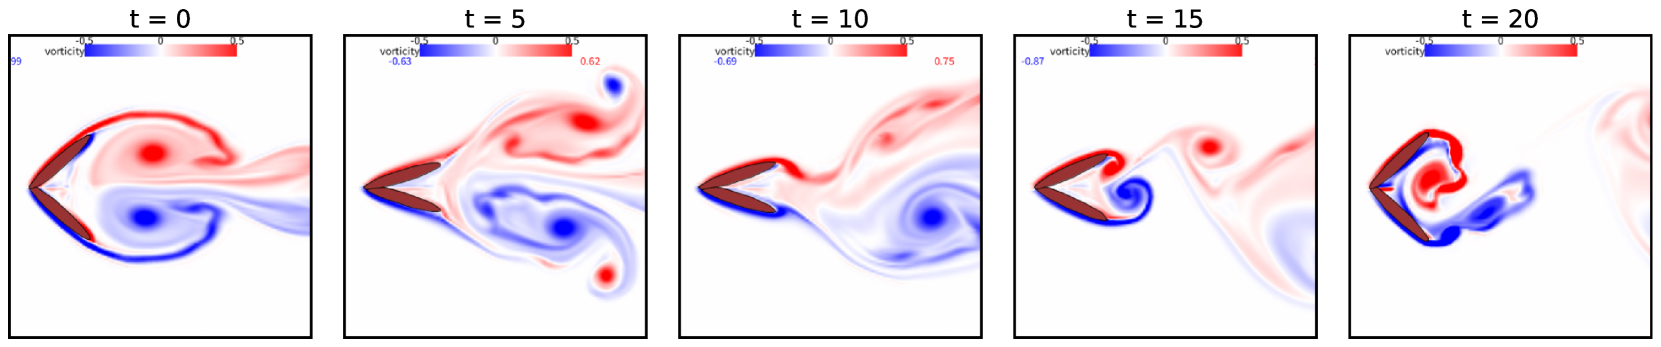
\includegraphics[height=0.8\textheight,width=1.05\textwidth,keepaspectratio]{images/science/generative-models-jellyfish.png}
        \caption*{See how the jellyfish moves and how the water flows around it, using DiffPhyCon.}
    \end{figure}

    \framebreak
    \begin{figure}
        \centering
        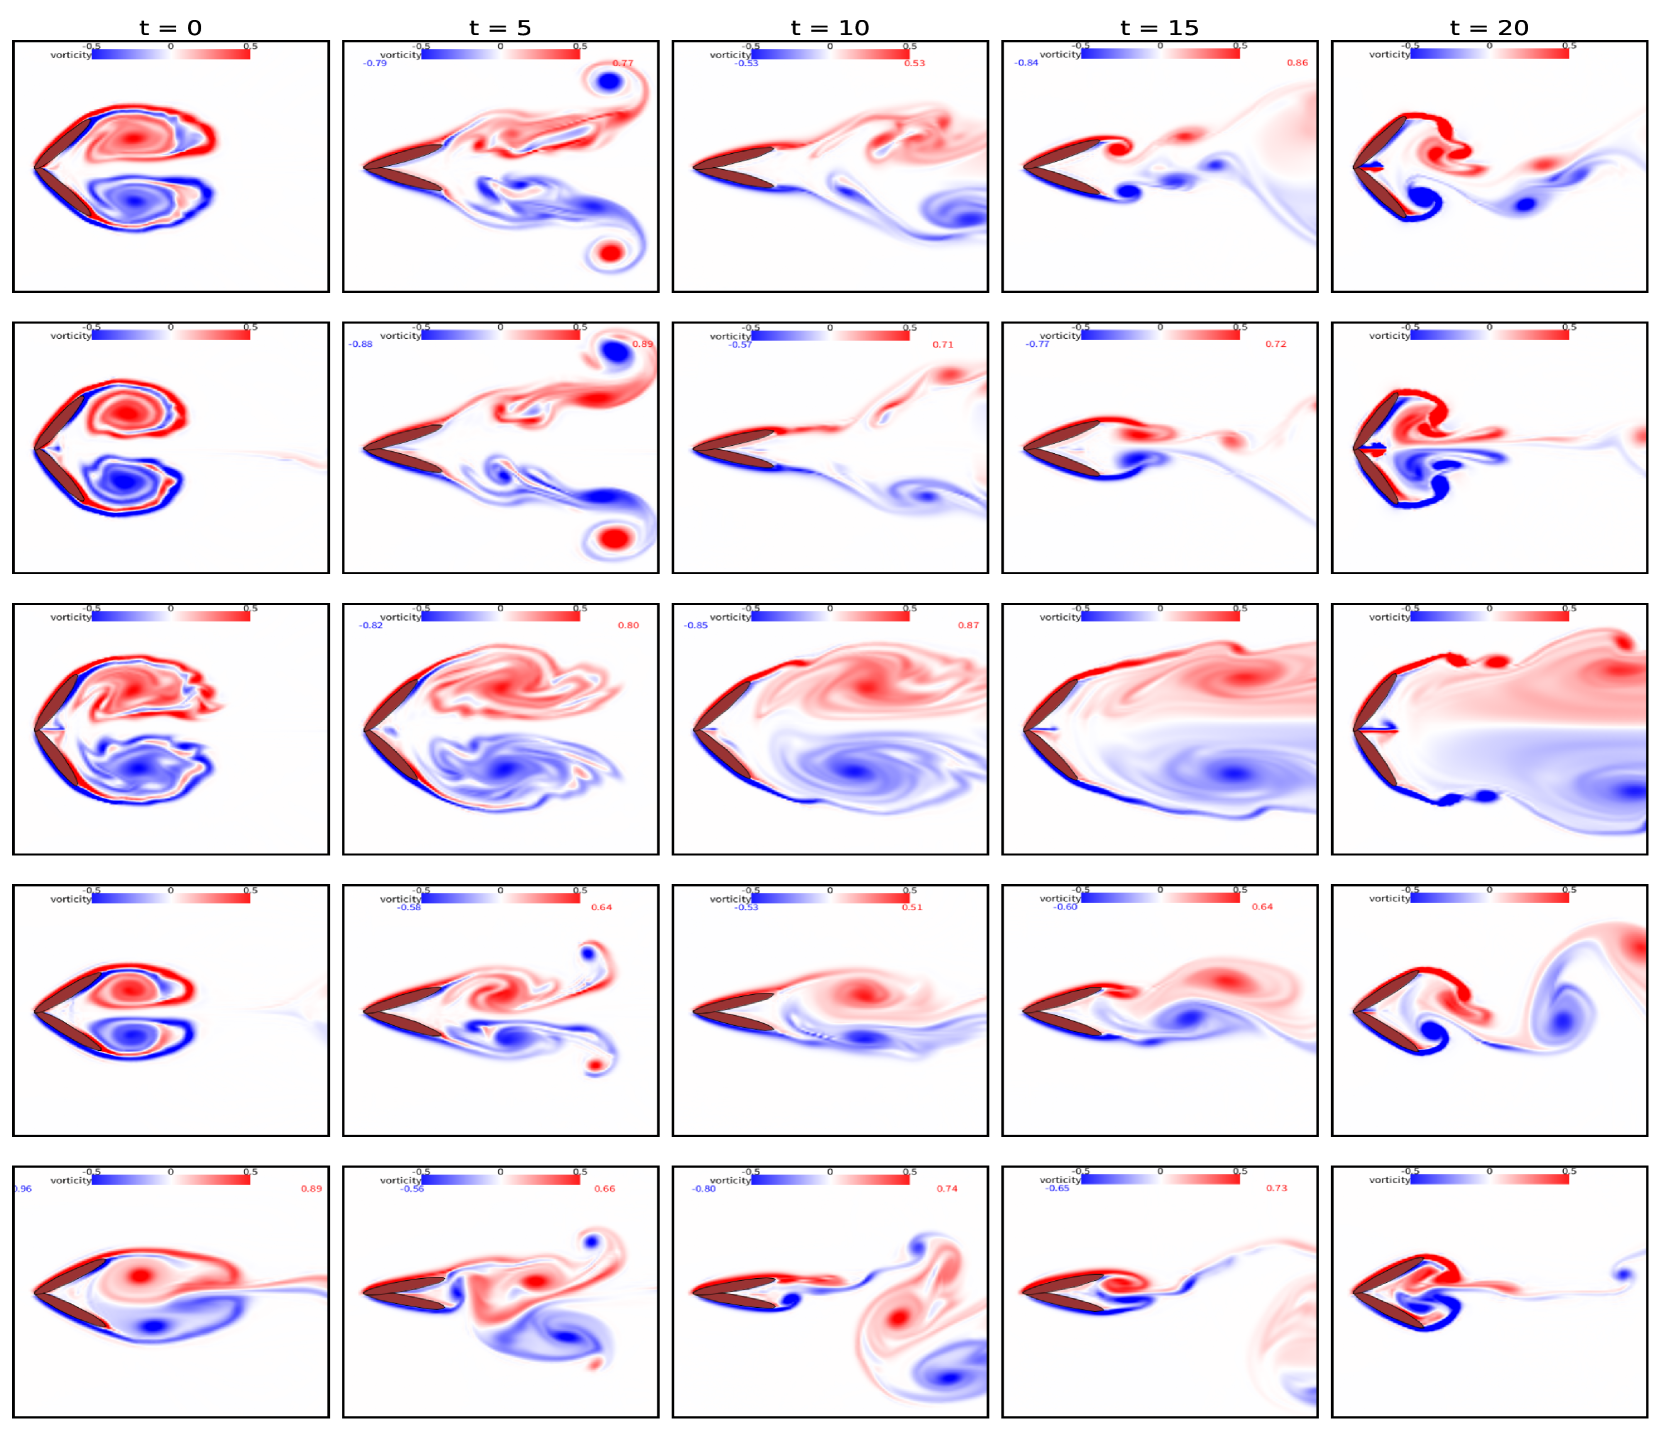
\includegraphics[height=0.9\textheight,width=1.05\textwidth,keepaspectratio]{images/science/generative-models-jellyfish-2.png}
    \end{figure}

    \framebreak
    \textbf{Challenges and Things to Watch Out For}
    \begin{itemize}
        \item \textbf{Needs Lots of Data:} Training these models often needs a lot of good data.
        \item \textbf{Complex Systems:} Some systems are so complicated that models struggle to learn them.
        \item \textbf{Hard to Understand:} It can be tricky to see why the model makes certain choices.
        \item \textbf{Still Needs Computers:} Even though it's faster, training and running these models can still use a lot of computer power.
        \item \textbf{Checking Results:} We must always check if the model's results match real experiments.
        \item \textbf{Follow the Laws of Physics:} The model should respect things like energy conservation to be realistic.
    \end{itemize}
\end{frame}